% This file was created with tikzplotlib v0.10.1.
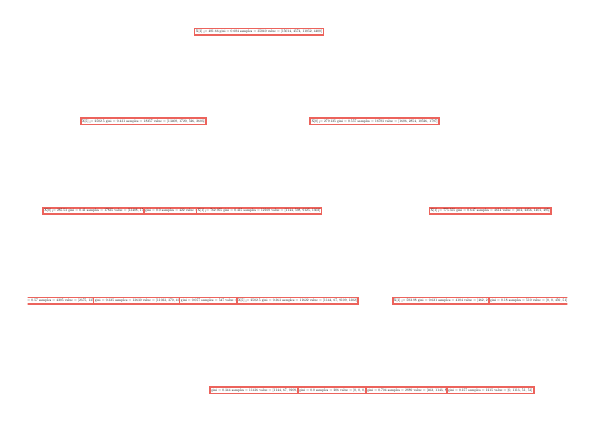
\begin{tikzpicture}

\definecolor{darkgray176}{RGB}{176,176,176}
\definecolor{tomato2369992}{RGB}{236,99,92}

\begin{axis}[
hide x axis,
hide y axis,
tick align=outside,
tick pos=left,
x grid style={darkgray176},
xmin=0, xmax=1,
xtick style={color=black},
y grid style={darkgray176},
ymin=0, ymax=1,
ytick style={color=black}
]
\draw (axis cs:0.428571428571429,0.1) node[
  scale=0.130016244214914,
  fill=white,
  draw=tomato2369992,
  line width=0.6pt,
  inner sep=3.6pt,
  text=black,
  rotate=0.0,
  align=center
]{gini = 0.344
samples = 11416
value = [1144, 67, 9109, 1096]};
\draw (axis cs:0.571428571428571,0.1) node[
  scale=0.130016244214914,
  fill=white,
  draw=tomato2369992,
  line width=0.6pt,
  inner sep=3.6pt,
  text=black,
  rotate=0.0,
  align=center
]{gini = 0.0
samples = 206
value = [0, 0, 0, 206]};
\draw (axis cs:0.714285714285714,0.1) node[
  scale=0.130016244214914,
  fill=white,
  draw=tomato2369992,
  line width=0.6pt,
  inner sep=3.6pt,
  text=black,
  rotate=0.0,
  align=center
]{gini = 0.704
samples = 2889
value = [462, 1143, 891, 393]};
\draw (axis cs:0.857142857142857,0.1) node[
  scale=0.130016244214914,
  fill=white,
  draw=tomato2369992,
  line width=0.6pt,
  inner sep=3.6pt,
  text=black,
  rotate=0.0,
  align=center
]{gini = 0.157
samples = 1215
value = [0, 1113, 51, 51]};
\draw (axis cs:0.0714285714285714,0.3) node[
  scale=0.130016244214914,
  fill=white,
  draw=tomato2369992,
  line width=0.6pt,
  inner sep=3.6pt,
  text=black,
  rotate=0.0,
  align=center
]{gini = 0.57
samples = 4205
value = [2375, 1350, 124, 356]};
\draw (axis cs:0.214285714285714,0.3) node[
  scale=0.130016244214914,
  fill=white,
  draw=tomato2369992,
  line width=0.6pt,
  inner sep=3.6pt,
  text=black,
  rotate=0.0,
  align=center
]{gini = 0.325
samples = 13630
value = [11033, 370, 402, 1825]};
\draw (axis cs:0.357142857142857,0.3) node[
  scale=0.130016244214914,
  fill=white,
  draw=tomato2369992,
  line width=0.6pt,
  inner sep=3.6pt,
  text=black,
  rotate=0.0,
  align=center
]{gini = 0.057
samples = 547
value = [0, 531, 16, 0]};
\draw (axis cs:0.5,0.3) node[
  scale=0.130016244214914,
  fill=white,
  draw=tomato2369992,
  line width=0.6pt,
  inner sep=3.6pt,
  text=black,
  rotate=0.0,
  align=center
]{X[5] <= 2502.5
gini = 0.363
samples = 11622
value = [1144, 67, 9109, 1302]};
\draw (axis cs:0.785714285714286,0.3) node[
  scale=0.130016244214914,
  fill=white,
  draw=tomato2369992,
  line width=0.6pt,
  inner sep=3.6pt,
  text=black,
  rotate=0.0,
  align=center
]{X[1] <= 582.98
gini = 0.621
samples = 4104
value = [462, 2256, 942, 444]};
\draw (axis cs:0.928571428571429,0.3) node[
  scale=0.130016244214914,
  fill=white,
  draw=tomato2369992,
  line width=0.6pt,
  inner sep=3.6pt,
  text=black,
  rotate=0.0,
  align=center
]{gini = 0.18
samples = 510
value = [0, 0, 459, 51]};
\draw (axis cs:0.142857142857143,0.5) node[
  scale=0.130016244214914,
  fill=white,
  draw=tomato2369992,
  line width=0.6pt,
  inner sep=3.6pt,
  text=black,
  rotate=0.0,
  align=center
]{X[0] <= 285.53
gini = 0.41
samples = 17835
value = [13408, 1720, 526, 2181]};
\draw (axis cs:0.285714285714286,0.5) node[
  scale=0.130016244214914,
  fill=white,
  draw=tomato2369992,
  line width=0.6pt,
  inner sep=3.6pt,
  text=black,
  rotate=0.0,
  align=center
]{gini = 0.0
samples = 422
value = [0, 0, 0, 422]};
\draw (axis cs:0.428571428571429,0.5) node[
  scale=0.130016244214914,
  fill=white,
  draw=tomato2369992,
  line width=0.6pt,
  inner sep=3.6pt,
  text=black,
  rotate=0.0,
  align=center
]{X[1] <= 762.955
gini = 0.415
samples = 12169
value = [1144, 598, 9125, 1302]};
\draw (axis cs:0.857142857142857,0.5) node[
  scale=0.130016244214914,
  fill=white,
  draw=tomato2369992,
  line width=0.6pt,
  inner sep=3.6pt,
  text=black,
  rotate=0.0,
  align=center
]{X[1] <= 775.555
gini = 0.647
samples = 4614
value = [462, 2256, 1401, 495]};
\draw (axis cs:0.214285714285714,0.7) node[
  scale=0.130016244214914,
  fill=white,
  draw=tomato2369992,
  line width=0.6pt,
  inner sep=3.6pt,
  text=black,
  rotate=0.0,
  align=center
]{X[5] <= 2502.5
gini = 0.431
samples = 18257
value = [13408, 1720, 526, 2603]};
\draw (axis cs:0.642857142857143,0.7) node[
  scale=0.130016244214914,
  fill=white,
  draw=tomato2369992,
  line width=0.6pt,
  inner sep=3.6pt,
  text=black,
  rotate=0.0,
  align=center
]{X[0] <= 279.125
gini = 0.557
samples = 16783
value = [1606, 2854, 10526, 1797]};
\draw (axis cs:0.428571428571429,0.9) node[
  scale=0.130016244214914,
  fill=white,
  draw=tomato2369992,
  line width=0.6pt,
  inner sep=3.6pt,
  text=black,
  rotate=0.0,
  align=center
]{X[1] <= 481.66
gini = 0.684
samples = 35040
value = [15014, 4574, 11052, 4400]};
\end{axis}

\end{tikzpicture}
